\documentclass[12pt, a4paper, dvipsnames]{report}

\usepackage[croatian]{babel}

\usepackage{csquotes}
\usepackage{fontspec}
\usepackage{fancyhdr}
\usepackage[left=2.5cm,top=2.5cm,right=2cm,bottom=2.5cm]{geometry}
\usepackage[onehalfspacing]{setspace}
\usepackage{graphicx}
\usepackage{minted}
\usepackage{enumitem}

\usepackage{lmodern}
\usepackage{tikz}
\usepackage{pgfplots}
\usepackage[binary]{SIunits}
\usepackage[european]{circuitikz}
\usetikzlibrary{arrows,arrows.meta,positioning,fit,shapes,calc,decorations.markings,decorations.text}

\usepackage{amsmath}

% For changing title styls with \titleformat
\usepackage[explicit]{titlesec}

% For Toc with dots
\usepackage{tocloft}

% For using hyperlinks
\usepackage{hyperref}

% Bibliography
\usepackage[backend=biber, sorting=none]{biblatex}
\addbibresource{bibliography.bib}

% Fancy header definition
\fancyhf{}

% Set page number in down-right corner of the page
\rfoot{\thepage}
\pagestyle{fancy}

% Also for pages with chapters.
\fancypagestyle{plain}{
    \fancyhf{}
    \fancyfoot[R]{\thepage}
}

% Remove default rule in header
\renewcommand{\headrulewidth}{0pt}

% Change section format style
\titleformat{\chapter}
    {\large\bfseries}{\thechapter.}{1em}{\MakeUppercase{#1}}
\titleformat{\section}
    {\large\bfseries}{\thesection}{0.5em}{#1}
\titleformat{\subsection}
    {\normalsize\bfseries}{\thesubsection}{0.5em}{#1}

\renewcommand\listingscaption{Ispis koda}

% Change section, subsection figure, table. listing numbering
\renewcommand{\thefigure}{\arabic{chapter}.\arabic{figure}.}
\renewcommand{\thetable}{\arabic{chapter}.\arabic{table}.}
\renewcommand{\theequation}{\arabic{chapter}-\arabic{equation}}
\renewcommand{\thelisting}{\arabic{chapter}.\arabic{listing}}


% Links style definitions
\hypersetup{
    % fits the width of the page to the window
    pdfstartview={FitH},
    pdftitle={Socket server za prijenos podataka iz postrojenja},
    pdfauthor={Damir Jelić},
    pdfkeywords={Arduino} {Haskell} {Daemon},
    % false: boxed links; true: colored links
    colorlinks=true,
    pdfborder={0,0,0},
    linkcolor=black,
    citecolor=OliveGreen,
    filecolor=Red,
    urlcolor=MidnightBlue,
}

% Source code coloring style
\usemintedstyle{friendly}

\begin{document}

\newpage
\begin{titlepage}
\begin{center}

\textbf{\MakeUppercase{\large
    Sveučilište Josipa Jurja Strossmayera u Osijeku}}\\[0.2cm]

\textbf{\MakeUppercase{\large Elektrotehnički fakultet}}\\[0.8cm]
\textbf{\large Sveučilišni studij}\\ [5cm]

\textbf{\MakeUppercase{\Large Nest socket server }}\\ [1cm]

\textbf{\large Diplomski rad}\\  [5 cm]

\textbf{\Large Damir Jelić}\\ [0.5cm]

\vfill

\textbf{\large Osijek, 2015.} \\

\end{center}
\end{titlepage}

\newpage
% Toc
%\renewcommand{\cftsecleader}{\cftdotfill{\cftdotsep}}
{\large\tableofcontents}
% Set Toc depth - so it doesn't show subsections
\addtocontents{toc}{\protect\setcounter{tocdepth}{1}}
% Removing page numbering from this page
\thispagestyle{empty}

\setcounter{page}{1}

\chapter{Uvod} \label{introduction}

Cilj je diplomskog rada ispitati mogućnost korištenja jeftinih mikroupravljača
za jednostavne poslove automatizacije te omogućiti udaljeno upravljanje
postrojenjem preko \emph{socket} \emph{servera}.

Kako bi se utvrdio cilj diplomskog rada, pomoću mikroupravljača je simulirano
postrojenje. Komunikacija prema računalu je ostvarena putem \emph{USB}
sučelja. Računalo šalje mikroupravljaču naredbe pomoću komunikacijskog
protokola. \emph{Socket} \emph{server} izrađen je tako da s jedne strane koristi
navedeni protokol da bi komunicirao s mikroupravljačem, a s druge strane
omogućuje klijentima upit u stanje postrojenja i postavljanje referentne
varijable postrojenja.

Za mikroupravljač odabran je \emph{Arduino Uno} koji preko USB-serijskog sučelja
i preko \emph{Firmata} protokola komunicira s računalom. Na \emph{Arduino}
spojena je vodena pumpa i senzor koji mjeri razinu vode u boci. Sustav od dvije
boce čini postrojenje, u jednoj boci održava se razina vode. Na računalu se
nalazi \emph{socket} \emph{server} pisan u \emph{Haskellu} koji upravlja
mikroupravljačem. Testni klijent pisan u \emph{Pythonu} spaja se na
\emph{server} te dohvaća mjernu veličinu (razinu vode u boci) i prikazuje
trenutno stanje sustava.

Rad je podijeljen u dva dijela. U prvom dijelu razrađene su teorijske
pretpostavke vezane uz temu. Važno je napomenuti kako je u ovom dijelu detaljno
opisan proces razvoj socket servera. Drugi dio bavi se implementacijom
postrojenja, regulatora, \emph{socket servera} i popratnog klijenta.

\newpage
\chapter{Pregled korištenih programskih jezika i idioma}

U ovom su poglavlju detaljno opisani programski jezici, tehnike i komunikacijski
protokoli koji su korištene pri izradi diplomskoga rada.

\begin{figure}[H]
\centering
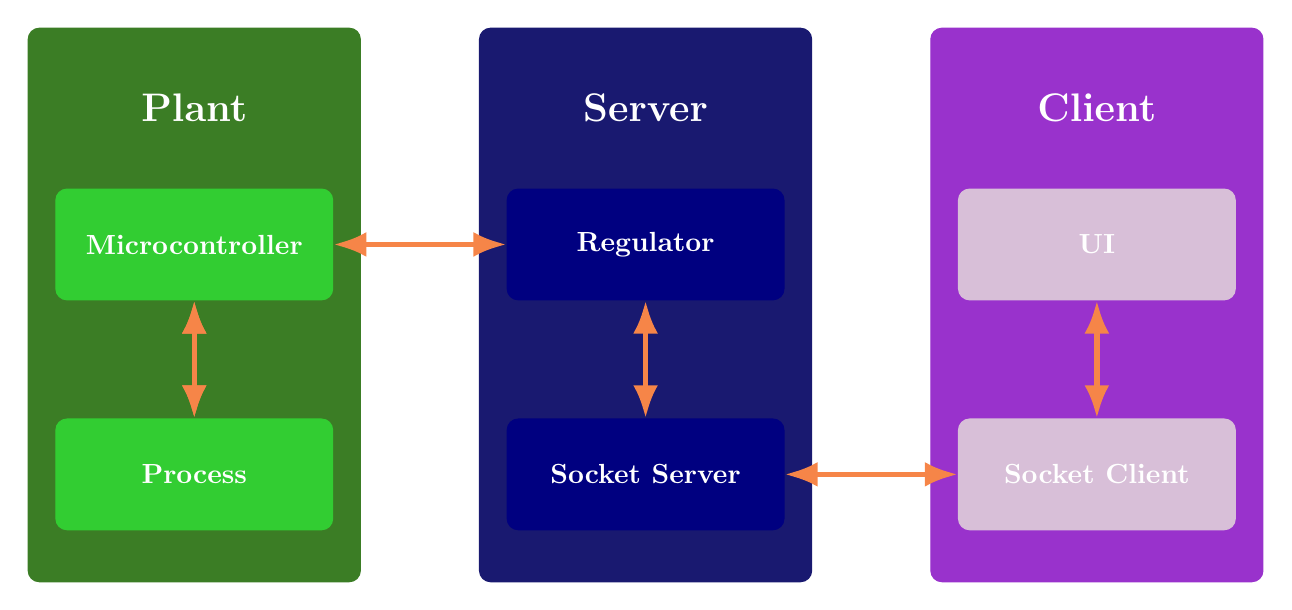
\begin{tikzpicture}
    \node[draw=OliveGreen, rectangle, minimum width=120, minimum height=200,
    label={[label distance=-180, font=\Large\bf, color=white]-90:Plant},
    fill=OliveGreen, rounded corners]
    (plant) {};

    \node[draw=MidnightBlue, rectangle, minimum width=120, minimum height=200,
    label={[label distance=-180, font=\Large\bf, color=white]-90:Server},
    fill=MidnightBlue, rounded corners, right=1.5 of plant]
    (daemon) {};

    \node[draw=DarkOrchid, rectangle, minimum width=120, minimum height=200,
    label={[label distance=-180, font=\Large\bf, color=white]-90:Client},
    fill=DarkOrchid, rounded corners, right=1.5 of daemon]
    (client) {};

    \node[draw=LimeGreen, rectangle, rounded corners, minimum height=40,
          minimum width=100, fill=LimeGreen, below=-5 of plant, font=\bf]
          (arduino) {\textcolor{white}{Microcontroller}};

    \node[draw=LimeGreen, rectangle, rounded corners, minimum height=40,
          minimum width=100, fill=LimeGreen, below=1.5 of arduino, font=\bf]
          (process) {\textcolor{white}{Process}};

    \node[draw=NavyBlue, rectangle, rounded corners, minimum height=40,
          minimum width=100, fill=NavyBlue, below=-5 of daemon, font=\bf]
          (regulator) {\textcolor{white}{Regulator}};

    \node[draw=NavyBlue, rectangle, rounded corners, minimum height=40,
          minimum width=100, fill=NavyBlue, below=1.5 of regulator, font=\bf]
          (sserver) {\textcolor{white}{Socket Server}};

    \node[draw=Thistle, rectangle, rounded corners, minimum height=40,
          minimum width=100, fill=Thistle, below=-5 of client, font=\bf]
          (UI) {\textcolor{white}{UI}};

    \node[draw=Thistle, rectangle, rounded corners, minimum height=40,
          minimum width=100, fill=Thistle, below=1.5 of UI, font=\bf]
          (sclient) {\textcolor{white}{Socket Client}};

    \draw[Latex-Latex, line width=2, color=Peach] (arduino) to (regulator);
    \draw[Latex-Latex, line width=2, color=Peach] (arduino) to (process);
    \draw[Latex-Latex, line width=2, color=Peach] (arduino) to (process);
    \draw[Latex-Latex, line width=2, color=Peach] (sserver) to (sclient);
    \draw[Latex-Latex, line width=2, color=Peach] (regulator) to (sserver);
    \draw[Latex-Latex, line width=2, color=Peach] (UI) to (sclient);
\end{tikzpicture}
\caption{Shematski prikaz rada}
\label{fig:main_sheme}
\end{figure}

Na slici \ref{fig:main_sheme} se vidi sinopsis diplomskoga rada koji je podijeljen u 3 dijela:
\begin{itemize}
        \item Postrojenje
        \item Server
        \item Klijent
\end{itemize}

Kao što je već spomenuto u poglavlju \ref{introduction} postrojenje sastoji se
od mikroupravljača i dviju boca koje služe kao model za održavanje razine vode.

Server koji je pisan u Haskell-u također se sastoji od dva dijela, regulatora i
socket server-a. Regulacijski dio s postrojenjem komunicira pomoću Firmata
protokola, a socket server s klijentima komunicira pomoću JSON-RPC protokola.

Klijent koji je pisan u Python-u sastoji se od korisničkog sučelja i socket
klijenta koji periodički dohvaća trenutno stanje postrojenja od servera.

\section{Haskell}

Haskell je moderan, standardan, nije striktan, čisto funkcionalan programski
jezik. Dizajniran je za širok spektar primjena, od numeričkih do
simboličkih \cite{haskell_intro}.

Haskell je nastao 1990. godine te nakon nekoliko godina razvoja glavne osobine
su mu bile \cite{haskell_history}:

\begin{itemize}
\item Statički pisan
\item Sigurnost tipova
\item Lijenost
\item Klase tipova.
\end{itemize}

Statički pisan jezik zahtijeva da pri kompilaciji koda svi tipovi podataka budu
poznati, što donosi niz prednosti kao primjećivanje grešaka prije nego što se
program izvrši, efikasniji kod jer compiler zna unaprijed veličinu podataka,
nije potrebno provjeravati tip podatka dok se program izvršava.

Sigurnost tipova proizlazi iz strogo statičkog pisanja, ona osigurava da
funkcije ne mogu primiti podatak pogrešnog tipa, takve će greške biti pri
kompilaciji prepoznate od strane compilera.

Lijenost (engl. \emph{Lazy evaluation}) je svojstvo jezika pri kojem se izrazi
evaluiraju tek kada je to potrebno, rezultat komputacije se računa tek kada je
on tražen negdje dalje. Lazy evaluation omogućuje elegantan rad sa beskonačnim
poljima. Moguće je definirati polje sa beskonačnim brojem članova, a da program
ne zauzme svu memoriju računala, pojedini će element liste biti evaluiran ako i
samo ako on njemu probamo pristupiti.

Klase tipova (engl. \emph{Type classes}) su nastale s ciljem omogućavanja
implementiranja preopterećenih aritmetičkih operatora i operatora jednakosti.

\subsection{Mrežno proramiranje}

Za mrežno programiranje Haskell nudi za modul
\mintinline{haskell}{Network.Socket} \cite{network_socket} koji korisniku
pruža sve standardne C funkcije za stvaranje UNIX socket-a.

\begin{figure}[H]
\centering

\begin{tikzpicture}[every node/.style = {font=\bf, rectangle, rounded corners,
                    minimum width=70},
                    connection/.style = {-Latex, Peach, line width=2}]
    \node[draw=OliveGreen, fill=OliveGreen]
          (socket) {\textcolor{white}{socket()}};

    \node[draw=MidnightBlue, fill=MidnightBlue, right=of socket]
          (bind) {\textcolor{white}{bind()}};

    \node[draw=Sepia, fill=Sepia, right=of bind]
          (listen) {\textcolor{white}{listen()}};

    \node[draw=DarkOrchid, fill=DarkOrchid, right=of listen]
          (accept) {\textcolor{white}{accept()}};

    \draw[connection] (socket) to (bind);
    \draw[connection] (bind)   to (listen);
    \draw[connection] (listen) to (accept);
\end{tikzpicture}
\caption{Programski tok izrade socket servera}
\label{fig:server_creation}
\end{figure}

Na slici \ref{fig:server_creation} je prikazan programski slijed izrade
socket server-a. Prvo se pomoću \mintinline{haskell}{socket} funckcije stvori
socket određenih karakteristika. U \mintinline{haskell}{Network.Socket} modulu
je ona definirana kao:
\mint{haskell}|socket :: Family -> SocketType -> ProtocolNumber -> IO Socket|

Iz definicije funkcije vidi se da je ona zapravo ista kao i standardna C
funkcija za stvaranje socket-a \cite[str.132]{unixnetwork}. Nakon što je stvoren
socket njemu se treba dodijeliti lokalna adresa odabranog protokola,
dodjeljivanje adrese postiže se s \mintinline{haskell}{bind} funkcijom čija
definicija glasi:
\mint{haskell}|bind :: Socket -> SockAddr -> IO ()|

Slijedi pretvaranje stvorenog socket-a u pasivni socket koji će čekati na ulazne
konekcije. To se ostvaruje pomoću funkcije \mintinline{haskell}{listen} koja je
definirana kao:
\mint{haskell}|listen :: Socket -> Int -> IO ()|

Na kraju je još potrebno pričekati konekciju klijenta što se ostvaruje s
funkcijom \mintinline{haskell}{accept} koja blokira daljni tok programa dok se
klijent ne spoji. Definicija funckije glasi:
\mint{haskell}|accept :: Socket -> IO (Socket, SockAddr)|
Funkcija nam vraća novi socket s pomoću kojim možemo razmjenjivati podatke s
klijentom i adresu klijenta. Razmjena se podataka može vršiti s
\mintinline{haskell}{sendTo} i \mintinline{haskell}{recvFrom} no radi
jednostavnosti možemo socket pretvoriti u handle te pisati i čitati podatke
kao da se radi o datoteci. Za to postoji \mintinline{haskell}{socketToHandle}
koja jednostavno primi socket i mode u kojem treba biti handle (read, write ili
oboje) i vrati handle. Definicija joj glasi:
\mint{haskell}|socketToHandle :: Socket -> IOMode -> IO Handle|

\subsection{Istodobnost}

Istodobnost (engl. \emph{Concurrency}) je svojstvo sustava kojim se istodobno
može izvršavati više računskih operacija ili komputacija.

Ekstenzija za istodobnost u Haskell-u se pojavila 1996. godine koja uvodi dva
nova idioma u Haskell \cite{concurrent}:
\begin{itemize}
        \item Procese i mehanizme za stvaranje procesa
        \item Atomarno promjenjivo stanje
\end{itemize}

Istodobnost u Haskell-u je uglavnom izvedena pomoću "Zelenih niti"
(engl.\emph{Green threads}). Zelene niti se ne izvršavaju u jezgri operativnog
sustava već u \emph{Haskell runtime-u}. Haskell ima hibridni višenitni
model kojim se N Haskell niti mogu vezivati na M niti operativnog sustava.

\begin{figure}[H]
\centering
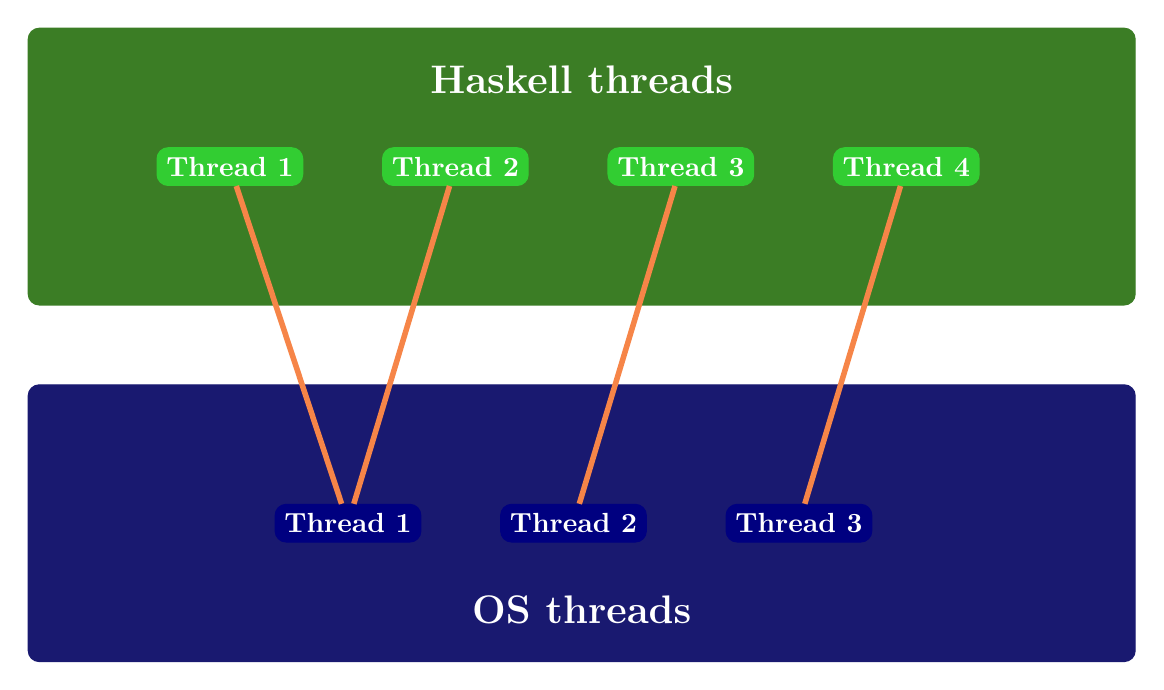
\begin{tikzpicture}
    \node[draw=OliveGreen, rectangle, minimum width=400, minimum height=100,
    label={[label distance=-90, font=\Large\bf, color=white]-90:Haskell threads},
    fill=OliveGreen, rounded corners]
    (hThreads) {};

    \node[draw=LimeGreen, rectangle, rounded corners,
          fill=LimeGreen, left=-3.5 of hThreads, font=\bf]
          (hThread1) {\textcolor{white}{Thread 1}};

    \foreach [count=\j from 1] \i in {2,...,4} {
        \node[draw=LimeGreen, rectangle, rounded corners,
              fill=LimeGreen, font=\bf, right=of hThread\j]
              (hThread\i) {\textcolor{white}{Thread \i}};
    }

    \node[draw=MidnightBlue, rectangle, rounded corners, minimum width=400,
          minimum height=100, below=of hThreads, label={[label distance=-90,
          font=\Large\bf, color=white]90:OS threads}, fill=MidnightBlue]
          (osThreads) {};

    \node[draw=NavyBlue, fill=NavyBlue, rectangle, rounded corners,
          left=-5.0 of osThreads, font=\bf] (osThread1)
          {\textcolor{white}{Thread 1}};

    \foreach [count=\j from 1] \i in {2,...,3} {
        \node[draw=NavyBlue, fill=NavyBlue, font=\bf, rectangle,
              rounded corners, right=of osThread\j]
              (osThread\i) {\textcolor{white}{Thread \i}};
    }

    \draw[line width=2, color=Peach] (hThread1) to (osThread1);
    \draw[line width=2, color=Peach] (hThread2) to (osThread1);
    \draw[line width=2, color=Peach] (hThread3) to (osThread2);
    \draw[line width=2, color=Peach] (hThread4) to (osThread3);
\end{tikzpicture}
\caption{N:M višenitni model Haskell-a}
\label{fig:thread_model}
\end{figure}

Na slici \ref{fig:thread_model} je prikazano kako se Haskell niti mapiraju na
niti operativnog sustava.
Interno se u Haskell-u stvaranje nove niti pretvara u alokaciju strukture koja
sprema trenutno stanje niti te se niti pretvaraju u jednu petlju.

Za stvaranje nove niti Haskell nudi \mintinline{haskell}{forkIO} funkciju koja
je dio \mintinline{haskell}{Control.Concurrent} modula
\cite{control_concurrent}, a definirana je kao:
\mint{haskell}|forkIO :: IO () -> IO ThreadId|

Što znači da funkcija prima kao prvi argument komputaciju (engl.
\emph{computation}) i vraća novu komputaciju koja kao rezultat proizvodi
\mintinline{haskell}{ThreadId} što nam služi kao referenca na novu nit koju će
funkcija stvoriti.

Osim niti za istodobno izvršavanje programa, bitna je i komunikacija između niti.
Za komunikaciju između niti Haskell nudi mutabilne dijeljene varijable zvane
\mintinline{haskell}{MVar} (Mutable Variables) koje se nalaze unutar
\mintinline{haskell}{Control.Concurrent.MVar} modula \cite{mvar}. One se mogu
koristiti na razne načine:

\begin{itemize}
\item Sinkronizirane mutabilne varijable.
\item Komunikacijski kanali između niti.
\item Binarni semafori.
\end{itemize}

Nova mutabilna varijabla koja sadrži podatak proizvoljnog tipa može se napraviti
s \mintinline{haskell}{newMVar}, definirana je kao:
\mint{haskell}|newMVar :: a -> IO (MVar a)|

Nakon što je varijabla stvorena, njom se može na razne načine manipulirati, između
ostalog može se zapisati novi podatak u nju, pročitati podatak ili zamijeniti s
nekim drugim podatkom.

Čitanje podatka bez njegove izmjene nam omogućuje
\mintinline{haskell}{readMVar}:
\mint{haskell}|readMVar :: MVar a -> IO a|

Za zamjenu podatka s nekim drugim postoji \mintinline{haskell}{swapMVar}
funkcija:
\mint{haskell}|swapMVar :: MVar a -> a -> IO a|

\newpage
\section{Python}

Python je interpretiran, objektno orijentiran, programski jezik visoke razine
s dinamičkom semantikom. Podatkovne strukture visoke razine i dinamičko pisanje
čine ga atraktivnim za vrlo brzo razvijanje aplikacija i za skriptni jezik za
spajanje više postojećih komponenti.
Python posjeduje jednostavnu i laku sintaksu koja povećava čitljivost i
olakšava održavanje software-a \cite{python_ref}.

\subsection{Mrežno programiranje}

Slično kao i Haskell, Python pruža sve standardne C funkcije za mrežno
programiranje. Sve se bitne funkcije nalaze u \mintinline{python}{Socket}
modulu \cite{python_socket}.

\begin{figure}[H]
\centering

\begin{tikzpicture}[every node/.style = {font=\bf, rectangle, rounded corners,
                    minimum width=70},
                    connection/.style = {-Latex, Peach, line width=2}]
    \node[draw=OliveGreen, fill=OliveGreen]
          (socket) {\textcolor{white}{socket()}};

    \node[draw=DarkOrchid, fill=DarkOrchid, right=of socket]
          (connect) {\textcolor{white}{connect()}};

    \draw[connection] (socket) to (connect);
\end{tikzpicture}
\caption{Programski tok izrade socket klijenta}
\label{fig:client_creation}
\end{figure}

Na slici \ref{fig:client_creation} je prikazan programski tok izrade socket
klijenta. Slično kao i sa serverom, prvo se stvori socket:
\mint{python}|socket.socket()|

Nakon stvaranja socketa potrebno ga je samo spojiti na serverski kraj socket-a:
\mint{python}|socket.connect()|

Nakon spajanja možemo socket pretvoriti \emph{file} objekt te čitati i pisati po
njemu kao da je datoteka:
\mint{python}|socket.makefile()|

Izrada socket-klijenta je daleko lakša od servera pogotovo jer se nerijetko ne
moramo brinuti o više istovremenih konekcija.

\newpage
\subsection{Urwid}

Urwid je Python biblioteka za izradu tekstualnih korisničkih sučelja. Urwid je
alternativna biblioteka standardnoj Curses biblioteci \cite{curses}, interno
koristi Curses biblioteku, no Urwid olakšava neke teže poslove pri izradi
tekstualnih sučelja \cite{urwid}.

Programi s Curses tekstualnim sučeljem često sliče programima s grafičkim
sučeljem koji posjeduju tekstualne kutije, razne forme za ispunjavanje, liste
s navigacijskim trakama i gumbe. Takvi grafički elementi ih mogu učiniti
lakšim za korištenje naspram standardnih tekstualnih programa, dok i dalje mogu
raditi na čisto tekstualnim uređajima. Programi s Curses tekstualnim sučeljem
također zahtijevaju manje resursa naspram grafičkih programa.

Urwid koristi događajnu petlju (engl. \emph{Event loop}) koja olakšava
rukovanje programskim ulazima i osvježavanje sučelja.

\subsection{Event loop}

Event loop je programski konstrukt koji čeka i otprema događaje ili poruke
unutar programa. Event loop šalje zahtjev pružatelju događaja (koji uglavnom
blokira sve dok neki događaj ne bude dostupan) te zatim poziva određenog
rukovatelja. Event loop je jedan od načina asinkronog programiranja.

\begin{figure}[H]
\centering
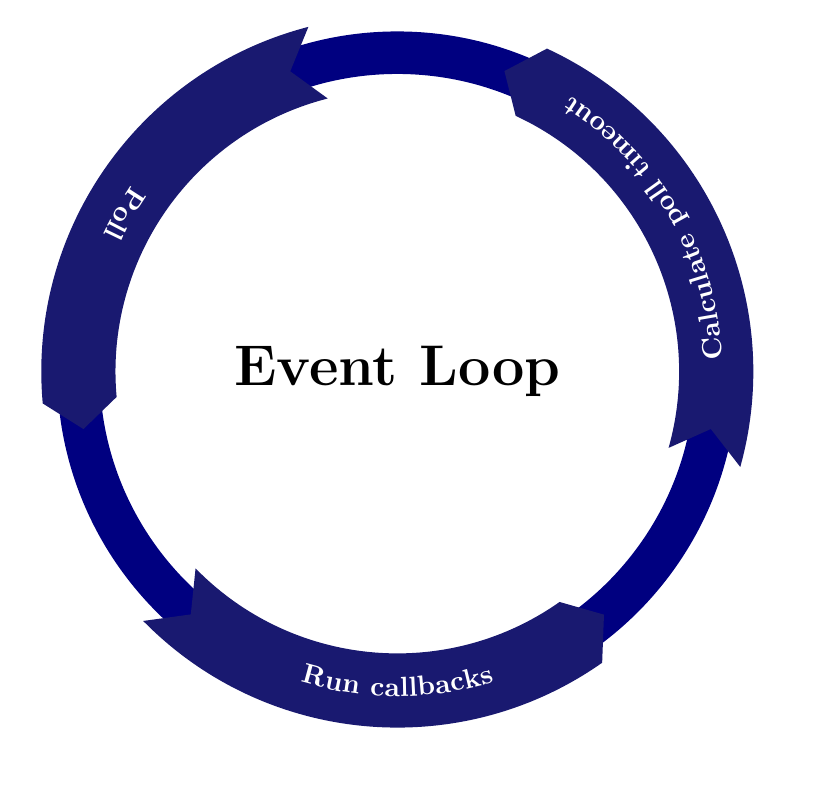
\begin{tikzpicture}[scale=0.9]
\newcommand{\arcarrow}[8]% inner radius, middle radius, outer radius, start angle, end angle, tip protusion angle, options, text
{   \pgfmathsetmacro{\rin}{#1}
    \pgfmathsetmacro{\rmid}{#2}
    \pgfmathsetmacro{\rout}{#3}
    \pgfmathsetmacro{\astart}{#4}
    \pgfmathsetmacro{\aend}{#5}
    \pgfmathsetmacro{\atip}{#6}
    \fill[#7] (\astart:\rin) arc (\astart:\aend:\rin) -- (\aend+\atip:\rmid) -- (\aend:\rout) arc (\aend:\astart:\rout) -- (\astart+\atip:\rmid) -- cycle;
    \path[decoration={text along path, text={|\color{white}\bf|#8}, text align={align=center}, raise=-0.5ex},decorate] (\astart+\atip:\rmid) arc (\astart+\atip:\aend+\atip:\rmid);
}

    \fill[even odd rule,NavyBlue] circle (4.8) circle (4.2);
    \draw (0, 0) node {\huge \bf Event Loop};

    \arcarrow {4}{4.5}{5}{325+20}{325+100}{5} {fill=MidnightBlue,
                draw=MidnightBlue, very thick} {Calculate poll timeout};
    \arcarrow {4}{4.5}{5}{85+20}{85+100}{5} {fill=MidnightBlue,
                draw=MidnightBlue, very thick} {Poll};
    \arcarrow {4}{4.5}{5}{205+20}{205+100}{5} {fill=MidnightBlue,
                draw=MidnightBlue, very thick} {Run callbacks};
\end{tikzpicture}
\caption{Event loop schematic}
\label{fig:event_loop}
\end{figure}

Na slici \ref{fig:event_loop} je prikazan programski tok Event loop-a. Prvo se
izračuna koliko će se čekati na događaj pa se pomoću Unix sistemskog poziva
\emph{poll} čeka na događaj te se na kraju poziva funkcija koja je namijenjena za
obradu određenog događaja.

\newpage
\section{Firmata}

Firmata je jednostavan MIDI baziran protokol koji je namijenjen za komunikaciju
računala s mikroupravljačem. Cilj mu je omogućiti direktno upravljanje što većim
dijelom mikroupravljača od strane računala.

Za podatkovni format protokola odabrane su MIDI \cite{midi} poruke. Nije u
potpunosti kompatibilan sa MIDI standardom pošto se koristi brža serijska
konekcija i poruke se ne preklapaju u svim slučajevima no za parsiranje poruka
moguće je koristiti postojeće MIDI parsere.

Protokol se može implementirati kao firmware za bilo koji mikroupravljač ili kao
software za računalo. Prva implementacija Firmate za mikroupravljače je bila za
Arduino obitelj mikroupravljača. Kao software za računalo postoji mnogo
Firmata implementacija za razne jezike između ostalog za Python \cite{pyfirmata}
i Haskell \cite{harduino}

\begin{table}[h]
\centering
    \begin{tabular}{|c|c|}
        \hline
        Naredba               & Numerička vrijednost \\
        \hline
        analog I/O message    & 0xE0 \\
        \hline
        digital I/O message   & 0x90 \\
        \hline
        report analog pin     & 0xC0 \\
        \hline
        report digital port   & 0xD0 \\
        \hline
        start sysex           & 0xF0 \\
        \hline
        set pin mode(I/O)     & 0xF4 \\
        \hline
        set digital pin value & 0xF5 \\
        \hline
        sysex end             & 0xF7 \\
        \hline
        protocol version      & 0xF9 \\
        \hline
        system reset          & 0xFF \\
        \hline
    \end{tabular}
    \caption{Firmata naredbe}
    \label{tbl:firmata}
\end{table}

Na tablici \ref{tbl:firmata} se vide neke od Firmata naredbi i njihove
odgovarajuće numeričke vrijednosti. Da bi se naredio reset mikroupravljača
jednostavno se preko serijske veze pošalje vrijednost 0xFF te nakon što
mikroupravljač primi poruku izvršit će reset rutinu.

\section{JSON-RPC}

JSON-RPC je jednostavan protokol za udaljene proceduralne pozive, ne sadržava
stanje i nije definiran kao transportan protokol \cite{jsonRPC}. Koristi JSON
\cite{jsonRFC} kao podatkovni format.

Pozivna poruka se sastoji od:
\begin{itemize}
        \item jsonrpc - verzija protokola
        \item method - ime udaljene metode koja se poziva
        \item params - ulazni parametri za metodu
        \item id - identifikacijska oznaka poruke
\end{itemize}

Ulazni parametri moraju biti strukturiran podatak, mogu biti u obliku niza ili
JSON objekt s imenovanim varijablama koje odgovaraju parametrima pozvane
metode.

Odgovor se sastoji od:
\begin{itemize}
    \item jsonrpc - verzija protokola ("2.0")
    \item result - rezultat koji vraća pozvana metoda
    \item error - greška ako ona postoji
    \item id - identifikacijska oznaka poruke
\end{itemize}

Ako dolazi do greške odgovor neće sadržavat rezultat, rezultat će biti
zamijenjen s greškom, svi ostali dijelovi odgovora ostaju isti.
Identifikacijska oznaka u odgovoru mora biti ista kao i u pozivu.

Primjer poziva:
\mint{json}|{"jsonrpc": "2.0", "method": "subtract", "params": [42, 23], "id": 1}|

Ovdje se vidi poziv koji koristi verziju 2.0 JSON-RPC protokola, poziva metodu
\emph{substract} kojoj predaje parametre u obliku niza (brojčane vrijednosti 42
i 23) te koristi identifikacijsku oznaku s brojem 1.

Primjer odgovora za prethodnu pozivnu poruku:
\mint{json}|{"jsonrpc": "2.0", "result": 19, "id": 1}|

U odgovoru se vidi da server koristi isti protokol kao klijent, vraća rezultat
pozvane metode te koristi istu identifikacijsku oznaku kao što je dobio u
pozivnoj poruci od klijenta.

\newpage
\chapter{Implementation}

U ovom poglavlju je objašnjena implementacija socket servera, odgovarajućeg
klijenta i na kraju samog postrojenja.

\newpage
\section{Server}

Arhitektura servera.

\begin{figure}[H]
\centering
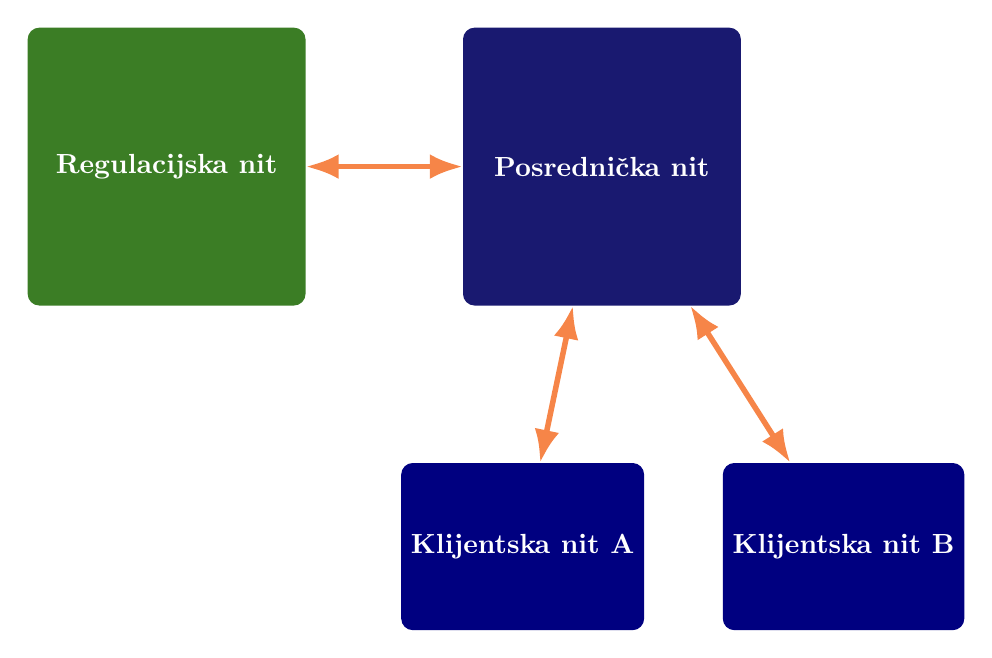
\begin{tikzpicture}[every node/.style = {font=\bf},
                    connection/.style = {Latex-Latex, Peach, line width=2}]
    \node[draw=OliveGreen,rectangle, rounded corners,
          fill=OliveGreen, minimum size=100]
          (regulator) {\textcolor{white}{Regulacijska nit}};

    \node[draw=MidnightBlue, rectangle, rounded corners, minimum size=100,
          right=2cm of regulator, fill=MidnightBlue]
          (server) {\textcolor{white}{Posrednička nit}};

    \node[draw=NavyBlue, rectangle, rounded corners,
          minimum size=60, below left=2cm and -2.3cm of server,
          fill=NavyBlue]
          (clientA) {\textcolor{white}{Klijentska nit A}};

    \node[draw=NavyBlue, rectangle, rounded corners,
          minimum size=60, right=of clientA,
          fill=NavyBlue]
          (clientB) {\textcolor{white}{Klijentska nit B}};

    \draw[connection] (regulator) to (server);
    \draw[connection] (server)    to (clientA);
    \draw[connection] (server)    to (clientB);
\end{tikzpicture}
\caption{Arhitektura servera}
\label{fig:architecture}
\end{figure}

Na slici \ref{fig:architecture} je prikazana komunikacija između pojedinih niti
unutar servera. Niti komuniciraju pomoću djeljenih varijabli.
... je dobro.

\begin{listing}[H]
\centering
\begin{minted}[frame=single]{haskell}
startDaemon :: Integer -> FilePath -> Bool -> IO ()
startDaemon port arduinoPort simulate = do
    sock <- socket AF_INET Stream 0

    bindSocket sock $ SockAddrInet (fromInteger port) iNADDR_ANY
    listen sock 50

    pv <- newMVar 0
    referenceChan <- newChan
    let com = ProcCom pv referenceChan

    _ <- forkIO $ mainLoop sock com

    controllerBroker arduinoPort simulate com
\end{minted}
\caption{Main entry point}
\label{lst:main}
\end{listing}

Na ispisu koda \ref{lst:main} je.

\begin{listing}[H]
\centering
\begin{minted}[frame=single]{haskell}
mainLoop :: Socket -> ProcCom PVType -> IO ()
mainLoop sock com = do
    (hdl, host, port) <- accept sock
    let hostinfo = host ++ ":" ++ show port
    noticeM rootLoggerName $ "Connected:    " ++ hostinfo
    _ <- forkIO $ runConn hdl com hostinfo

    mainLoop sock com
\end{minted}
\caption{Server mainloop}
\label{lst:mainloop}
\end{listing}

\begin{listing}[H]
\centering
\begin{minted}[frame=single]{haskell}
runConn :: Handle -> ProcCom PVType -> String -> IO ()
runConn hdl com hostinfo = do
    isEof <- hIsEOF hdl

    if isEof then do
        hClose hdl
        noticeM rootLoggerName $ "Disconnected: " ++ hostinfo
    else do
        contents <- hGetLine hdl
        debugM rootLoggerName $ "RPC request : " ++ contents

        response <- handleMsg com $ C.pack contents
        debugM rootLoggerName $ "RPC response: " ++ C.unpack response

        C.hPutStrLn hdl response
\end{minted}
\caption{Client handler thread}
\label{lst:client handler}
\end{listing}

\begin{listing}[H]
\centering
\begin{minted}[frame=single]{haskell}
controllerBroker :: FilePath -> Bool -> ProcCom PVType -> IO ()
controllerBroker arduinoPort simulate (ProcCom pvMVar refChan) = do
    refMVar <- newMVar 0

    _ <- forkIO $ forever $ do
            ref <- readChan refChan
            swapMVar refMVar ref

    if simulate then
        simulatorLoop refMVar pvMVar
    else do
        controlLoop arduinoPort refMVar pvMVar
        shutDownArduino arduinoPort

    noticeM rootLoggerName "Shutting daemon down."
\end{minted}
\caption{Controler broker}
\label{lst:controler broker}
\end{listing}

\subsection{Regulator}

\begin{listing}[H]
\centering
\begin{minted}[frame=single]{haskell}
forever $ do
    integral  <- liftIO $ takeMVar integralMVar
    reference <- liftIO $ readMVar refMVar

    sensorValue <- analogRead sensor
    let fillHeight = sensorValueFunc sensorValue
    _ <- liftIO $ swapMVar pvMVar fillHeight

    let error = reference - fillHeight

    let proportional_term = kp * error
    let integral_term     = integral + ki * error / sampleTime

    let output = clampAndScaleOutput $ proportional_term + integral_term

    analogWrite pwm_pin output
    delay sampleTime
\end{minted}
\caption{Regulacijska petlja}
\label{lst:regulator}
\end{listing}

\newpage
\section{Client}
\begin{listing}[H]
\centering
\begin{minted}[frame=single]{python}
def main():
    sock = socket.socket(socket.AF_INET, socket.SOCK_STREAM)
    sock.connect((args.host, args.port))

    tank = TankWidget()
    command_line = CommandLine(cmd_list, remote_cmds, sock)
    top = urwid.Frame(tank, None, command_line, 'footer')

    evl = urwid.AsyncioEventLoop(loop=asyncio.get_event_loop())
    loop = urwid.MainLoop(top, palette, event_loop=evl)

    loop.watch_file(sock.fileno(), read_cb)
    loop.set_alarm_in(0.1, periodic_tasks)

    loop.run()
\end{minted}
\caption{Client main loop}
\label{lst:client main}
\end{listing}

\begin{listing}[H]
\centering
\begin{minted}[frame=single]{python}
    def periodic_tasks(loop, data):
        request , _ = lvl_cmd('update-tank', [])
        try:
            sock.send(bytes(request, 'utf-8'))
        except BrokenPipeError as e:
            pass

        tank.update()

        loop.set_alarm_in(args.interval, periodic_tasks)

    loop.watch_file(sock.fileno(), read_cb)
\end{minted}
\caption{Periodic update dings}
\label{lst:periodic tasks}
\end{listing}


\newpage
\newpage
\section{Postrojenje}

\begin{figure}[H]
\centering
\includegraphics[scale=0.80]{figures/shield_schematic.pdf}
\caption{Električna shema postrojenja}
\end{figure}

\newpage
\subsection{Matematički model postrojenja}

\begin{equation} \frac{dV}{dt} = q_{in} - q_{out} \end{equation}

\begin{equation} q_{out} = a \sqrt{2gh} \end{equation}

\begin{equation} q_{in} = k_p V \end{equation}

\begin{equation} A\frac{dh}{dt} = k_p V - a \sqrt{2gh} \end{equation}

\begin{equation} \frac{d\delta h}{dt} = \frac{k_p}{A} \delta V -
                 \frac{a \sqrt{2g}}{2 A \sqrt{h_0}} \delta h \end{equation}

\begin{equation} \frac{d\delta h}{dt} = k_1 \delta V
                 - k_2 \delta h \end{equation}

\begin{equation} s H(s) = k_1 V(s) - k_2 H(s) \end{equation}

\begin{equation} H(s)(s+k_2) = k_1 V(s) \end{equation}

\begin{equation} G(s) = \frac{H(s)}{V(s)} = \frac{k_1}{s+k_2} \end{equation}

\begin{figure}[H]
\centering
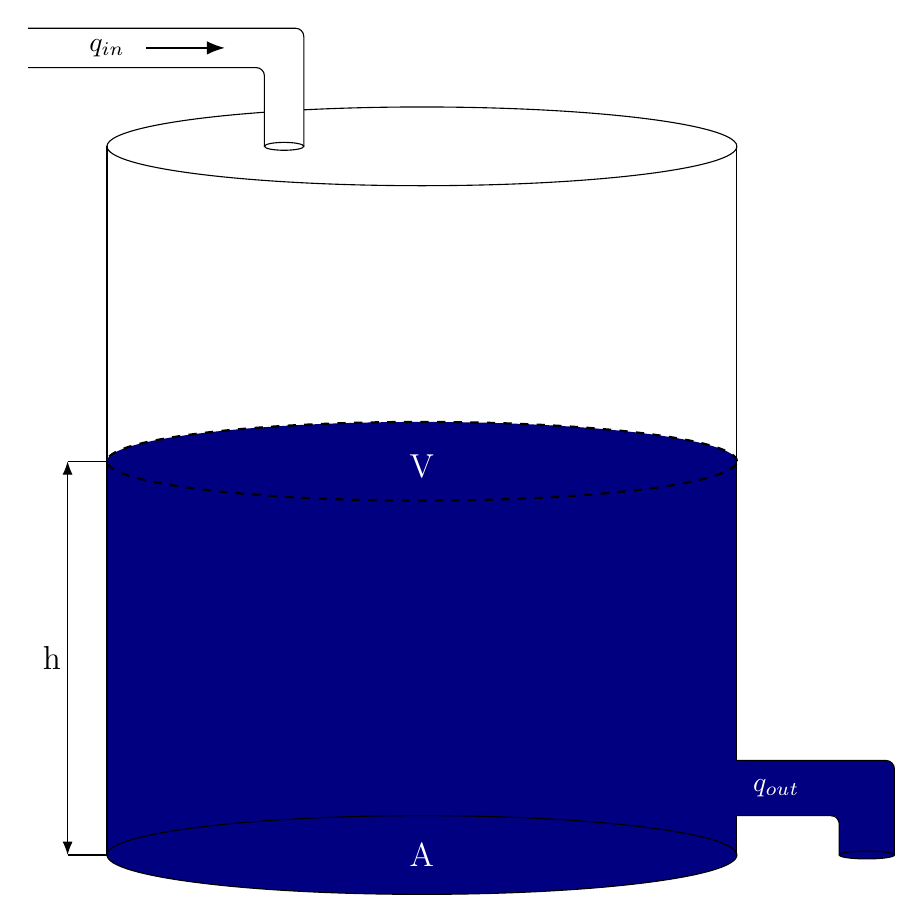
\begin{tikzpicture}[every node/.style = {font = \footnotesize}]
    \tikzset{weird fill/.style={append after command={
    \pgfextra
        \draw [#1, sharp corners, fill=#1]%
        (\tikzlastnode.west)%
        [rounded corners=0] |- (\tikzlastnode.north)%
        [rounded corners=3] -| (\tikzlastnode.east)%
        [rounded corners=0] |- (\tikzlastnode.south)%
        [rounded corners=0] -| (\tikzlastnode.west);
        \endpgfextra}}}

    \draw [rounded corners=3] (-5,10) -- (-2,10) -- (-2,9);
    \draw [rounded corners=3] (-5,10.5) -- (-1.5,10.5) -- (-1.5,9);
    \draw (-1.75, 9) circle [x radius=0.25, y radius=0.05];
    \draw (-4, 10.25) node [font=\normalsize] {$q_{in}$};
    \draw [-Latex, thick] (-3.5, 10.25) -- (-2.5, 10.25);

    \draw (0, 2.5) node[rectangle, minimum width=228, minimum height=140,
    fill=NavyBlue] {};

    \draw [fill=NavyBlue] (0,0) circle [x radius=4, y radius=0.5];
    \draw [fill=NavyBlue, thick, dashed] (0,5) circle [x radius=4, y radius=0.5];

    \node [font=\large] (area) {\textcolor{white}{A}};
    \node [font=\large, above=4.4 of area] {\textcolor{white}{V}};

    \draw (4,9)  arc[x radius = 4, y radius = 0.5, start angle=0, end angle=112];
    \draw (4,9)  arc[x radius = 4, y radius = 0.5, start angle=0, end angle=-240];

    \draw (-4,0)  -- (-4,9);
    \draw (4,0)   -- (4,0.5);
    \draw (4,1.2) -- (4,9);

    \draw (4.9, 0.85)
    node[weird fill=NavyBlue, rectangle, minimum width=62, minimum height=19]
    (qout1) {};
    \draw (4.5, 0.85) node [font=\normalsize] {\textcolor{white}{$q_{out}$}};

    \node [below right=-0.1 and -0.7 of qout1, fill=NavyBlue, minimum width=20, minimum
    height=17] (qout2) {};

    \draw [NavyBlue, fill=NavyBlue] (5.2, 0.6) -- (5.2,0.7) -- (5.5,0.7) -- (5.30, 0.4);
    \draw [NavyBlue, fill=NavyBlue] (5.2, 0.6) -- (5.2,0.5) -- (5.5,0.49);
    \draw [rounded corners=3] (4,1.2) -- (6,1.2) -- (6,0);
    \draw [rounded corners=3] (4,0.5) -- (5.3,0.5) -- (5.3,0);

    \draw [fill=NavyBlue] (5.65,0) circle [x radius=0.35, y radius=0.05];

    \draw (-4, 0) -- (-4.5, 0);
    \draw (-4, 5) -- (-4.5, 5);
    \draw [Latex-Latex] (-4.5, 0) -- (-4.5, 5);
    \draw (-4.7, 2.5) node [font=\large] {h};

\end{tikzpicture}
\caption{Shematski model postrojenja}
\end{figure}

\newpage
\chapter{Zaključak}

U radu je razvijen i predstavljen socket server za komunikaciju s postrojenjem.
Server komunicira s Arduino mikroupravljačkom pločicom i upravlja postrojenjem
koje je spojeno na pločicu. Demonstrirano je uspješno automatsko upravljanje
razine vode u spremniku. Razvijen je i klijent koji u stvarnom vremenu daje uvid
u stanje postrojenja te omogućuje udaljenu promjenu regulirane veličine. Tijekom
izrade, glavni problemi bili su omogućavanje istovremenog obavljanja poslova
regulacije i posluživanja podataka udaljenim klijentima, izrada makete
postrojenja te povezivanje svih dijelova rada u cjelinu.

Predstavljeno riješenje koje koristi regulator unutar socket servera ima svoje
prednosti i nedostatke. Nedostatci su vezani uz brzinu regulacije, zbog
serijskog protokola koji je korišten za komunikaciju postrojenja i socket
servera nije moguće regulirati procese koji imaju jako ograničene vremenske
zahtjeve. Zahtjev za dodatnim računalom pored mikroupravljača za obavljanje
posla regulacije također je jedan nedostatak. Prednosti su mogućnost rapidnog
razvoja regulatora, mogućnost izmjene regulatora bez ponovnog programiranja
mikroupravljača, mogućnost udaljenog upravljanja postrojenjem te fleksibilnost.

Široka dostupnost jeftinih mikroupravljača te malih računalnih platformi
omogućuje korištenje predstavljenog rješenja u razne svrhe kućne
automatizacije. Moguća je izrada mreže automatizirnih procesa kojima je
omogućeno daljinsko upravljanje pomoću socket servera.

Riješenje također ima visoki potencijal za poboljšanja. Moguće je poboljšati
parametre regulatora te ostvariti bolje upravljanje, prebaciti regulator na
mikroupravljač te tako smanjiti latenciju. Na serveru se lako mogu
implementirati razne vrste regulatora te bi se one mogle dinamički izmjenjivati.
Komunikacija klijenta i servera izvršava se nekriptiran. Na serveru
se također može implementirati zahtjev za autentikacijom prije nego se dozvoli uvid u
stanje postrojenja.


% No page numbers from here on.
\renewcommand{\thepage}{}

\printbibliography[heading=bibintoc, title=Literatura]

\newpage

\chapter*{Sažetak}
\addcontentsline{toc}{chapter}{Sažetak}
Pojavom jeftinih mikroupravljača i mini računala mogućnosti povezivanja
fizikalnog svijeta s digitalnim postaju sve veće.
Svrha diplomskog rada je ispitivanje mogućnost korištenja jeftinih mikroupravljača
za jednostavne poslove automatizacije kao i udaljenog upravljanja postrojenja 
preko \emph{socket} \emph{servera}.

Za mikroupravljač \emph{Arduino Uno} preko USB-serijskog sučelja i preko \emph{Firmata} 
protokola komunicira s računalom. Na njega je je vodena pumpa i senzor koji mjeri 
razinu vode u boci te sustav od dvije boce. Na računalu se nalazi \emph{socket} \emph{server} 
pisan u \emph{Haskellu} koji upravlja mikroupravljačem. Testni klijent pisan u 
\emph{Pythonu} spaja se na \emph{server} te dohvaća mjernu veličinu 
i prikazuje trenutno stanje sustava.

Rad je podijeljen u dva dijela: teorijski dio koji detaljno opisuje proces razvoja socket 
servera te praktični dio koji se bavi implementacijom postrojenja, regulatora, \
emph{socket servera} i popratnog klijenta.
\\

\noindent\textbf{Ključne riječi:} Haskell, Arduino, Automatizacija,
Python, Socket server, Firmata
\chapter*{Abstract}
The rise of cheap microcontrollers and mini computers have enabled new possibilities
of connecting the physical world with the digital.
The purpose of this paper is to explore the possibilities of cheap microcontrollers 
for simple automation as well as to enable remote control using a socket server.

The microcontroller Arduino Uno was chosen which communicates through the USB 
interface and the  Firmata protocol with the computer. A water pump and a sensor, 
which measures the water level, were connected as well as two bottles. 
The computer is equipped with a socket server written in Haskell 
which controls the microcontroller. The test client written in Python is being 
connected to the server and pumps the requested amount of water and shows the 
current system status.

The paper is divided into two parts. The first part shall elaborate the theoretical presuppositions 
regarding the subject matter. The second shall address the implementation of the system, 
the regulators, the socket servera and the accompanying client.
\\

\noindent\textbf{Keywords} Haskell, Arduino, Automation,
Python, Socket server, Firmata

\newpage

\chapter*{Životopis}
\addcontentsline{toc}{chapter}{Životopis}

Damir Jelić rođen je 8.~ožujka 1989.~godine u Osijeku. Osnovno
obrazovanje stekao je u osnovnoj školi Šećerana u Šećerani. Nakon toga,
pohađao je Prvu srednju školu u Belom Manastiru, smjer Tehničar za računalstvo,
2007. godine polaže maturu i iste godine upisuje Preddiplomski studij
Računarstva na Elektrotehničkom fakultetu u Osijeku. 2010. godine završava
Preddiplomski studij računarstva te upisuje Diplomski studij Procesnog
računarstva. Dva puta je sudjelovao u programu Google Summer of Code: oba puta u
sklopu PulseAudio organizacije, gdje je radio na dinamičkom podešavanju latencije
i \emph{resampling} poboljšanjima za PulseAudio softverski projekt.

\vspace{1cm}
\noindent \vspace*{1.0cm} \makebox[1.5in]{\hrulefill}

\chapter*{Prilozi}
\addcontentsline{toc}{chapter}{Prilozi}

\section*{Prikaz spremnika sa senzorom}

\begin{figure}[h]
\centering
\includegraphics[angle=-90, scale=0.4]{figures/tank_picture_resized.jpeg}
\end{figure}

\newpage
\section*{Prikaz Arduina i popratnog \emph{shielda}}

\begin{figure}[h]
\centering
\includegraphics[angle=90, scale=0.4]{figures/shield_picture_resized.jpeg}
\end{figure}


\end{document}
